

\tikzset{every picture/.style={line width=0.75pt}} %set default line width to 0.75pt        

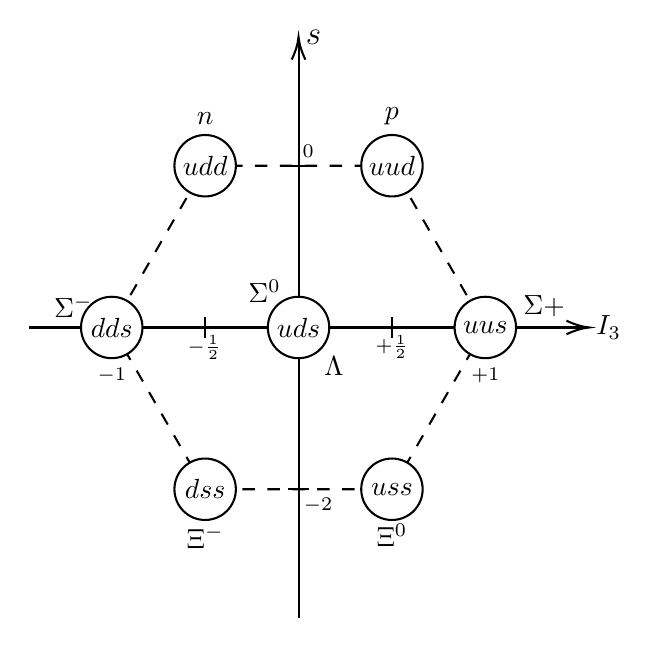
\begin{tikzpicture}[x=0.75pt,y=0.75pt,yscale=-1,xscale=1]
%uncomment if require: \path (0,585); %set diagram left start at 0, and has height of 585

%Shape: Regular Polygon [id:dp3461512214390913] 
\draw  [dash pattern={on 4.5pt off 4.5pt}] (360,280) -- (315,357.94) -- (225,357.94) -- (180,280) -- (225,202.06) -- (315,202.06) -- cycle ;
%Straight Lines [id:da7975119261953387] 
\draw    (140,280) -- (408,280) ;
\draw [shift={(410,280)}, rotate = 180] [color={rgb, 255:red, 0; green, 0; blue, 0 }  ][line width=0.75]    (10.93,-3.29) .. controls (6.95,-1.4) and (3.31,-0.3) .. (0,0) .. controls (3.31,0.3) and (6.95,1.4) .. (10.93,3.29)   ;
%Straight Lines [id:da49187250319695275] 
\draw    (270,420) -- (270,142) ;
\draw [shift={(270,140)}, rotate = 90] [color={rgb, 255:red, 0; green, 0; blue, 0 }  ][line width=0.75]    (10.93,-3.29) .. controls (6.95,-1.4) and (3.31,-0.3) .. (0,0) .. controls (3.31,0.3) and (6.95,1.4) .. (10.93,3.29)   ;
%Straight Lines [id:da04662903115423256] 
\draw    (225,275) -- (225,285) ;
%Straight Lines [id:da6078809997154113] 
\draw    (315,275) -- (315,285) ;
%Shape: Circle [id:dp2506066338504991] 
\draw  [fill={rgb, 255:red, 255; green, 255; blue, 255 }  ,fill opacity=1 ] (210.2,202.06) .. controls (210.2,193.88) and (216.83,187.26) .. (225,187.26) .. controls (233.17,187.26) and (239.8,193.88) .. (239.8,202.06) .. controls (239.8,210.23) and (233.17,216.86) .. (225,216.86) .. controls (216.83,216.86) and (210.2,210.23) .. (210.2,202.06) -- cycle ;
%Shape: Circle [id:dp49323091495562255] 
\draw  [fill={rgb, 255:red, 255; green, 255; blue, 255 }  ,fill opacity=1 ] (300.2,202.06) .. controls (300.2,193.88) and (306.83,187.26) .. (315,187.26) .. controls (323.17,187.26) and (329.8,193.88) .. (329.8,202.06) .. controls (329.8,210.23) and (323.17,216.86) .. (315,216.86) .. controls (306.83,216.86) and (300.2,210.23) .. (300.2,202.06) -- cycle ;
%Shape: Circle [id:dp2780130541001513] 
\draw  [fill={rgb, 255:red, 255; green, 255; blue, 255 }  ,fill opacity=1 ] (165.2,280) .. controls (165.2,271.83) and (171.83,265.2) .. (180,265.2) .. controls (188.17,265.2) and (194.8,271.83) .. (194.8,280) .. controls (194.8,288.17) and (188.17,294.8) .. (180,294.8) .. controls (171.83,294.8) and (165.2,288.17) .. (165.2,280) -- cycle ;
%Shape: Circle [id:dp22149042815123876] 
\draw  [fill={rgb, 255:red, 255; green, 255; blue, 255 }  ,fill opacity=1 ] (345.2,280) .. controls (345.2,271.83) and (351.83,265.2) .. (360,265.2) .. controls (368.17,265.2) and (374.8,271.83) .. (374.8,280) .. controls (374.8,288.17) and (368.17,294.8) .. (360,294.8) .. controls (351.83,294.8) and (345.2,288.17) .. (345.2,280) -- cycle ;
%Shape: Circle [id:dp2315285626329665] 
\draw  [fill={rgb, 255:red, 255; green, 255; blue, 255 }  ,fill opacity=1 ] (210.2,357.94) .. controls (210.2,349.77) and (216.83,343.14) .. (225,343.14) .. controls (233.17,343.14) and (239.8,349.77) .. (239.8,357.94) .. controls (239.8,366.12) and (233.17,372.74) .. (225,372.74) .. controls (216.83,372.74) and (210.2,366.12) .. (210.2,357.94) -- cycle ;
%Shape: Circle [id:dp3088315424845015] 
\draw  [fill={rgb, 255:red, 255; green, 255; blue, 255 }  ,fill opacity=1 ] (300.2,357.94) .. controls (300.2,349.77) and (306.83,343.14) .. (315,343.14) .. controls (323.17,343.14) and (329.8,349.77) .. (329.8,357.94) .. controls (329.8,366.12) and (323.17,372.74) .. (315,372.74) .. controls (306.83,372.74) and (300.2,366.12) .. (300.2,357.94) -- cycle ;
%Shape: Circle [id:dp27152267435822064] 
\draw  [fill={rgb, 255:red, 255; green, 255; blue, 255 }  ,fill opacity=1 ] (255.2,280) .. controls (255.2,271.83) and (261.83,265.2) .. (270,265.2) .. controls (278.17,265.2) and (284.8,271.83) .. (284.8,280) .. controls (284.8,288.17) and (278.17,294.8) .. (270,294.8) .. controls (261.83,294.8) and (255.2,288.17) .. (255.2,280) -- cycle ;
%Straight Lines [id:da5232366045305828] 
\draw    (265,202.1) -- (275,202.1) ;
%Straight Lines [id:da5088485977717139] 
\draw    (265,357.94) -- (275,357.94) ;

% Text Node
\draw (272,140) node [anchor=west] [inner sep=0.75pt]  [font=\large]  {$s$};
% Text Node
\draw (412,280) node [anchor=west] [inner sep=0.75pt]    {$I_{3}$};
% Text Node
\draw (270.5,190.65) node [anchor=north west][inner sep=0.75pt]  [font=\fontsize{0.71em}{0.85em}\selectfont]  {$0$};
% Text Node
\draw (271.08,360.57) node [anchor=north west][inner sep=0.75pt]  [font=\fontsize{0.71em}{0.85em}\selectfont]  {$-2$};
% Text Node
\draw (180,298.2) node [anchor=north] [inner sep=0.75pt]  [font=\fontsize{0.71em}{0.85em}\selectfont]  {$-1$};
% Text Node
\draw (360,298.2) node [anchor=north] [inner sep=0.75pt]  [font=\fontsize{0.71em}{0.85em}\selectfont]  {$+1$};
% Text Node
\draw (315.09,282.28) node [anchor=north] [inner sep=0.75pt]  [font=\fontsize{0.71em}{0.85em}\selectfont]  {$+\frac{1}{2}$};
% Text Node
\draw (224.65,282.6) node [anchor=north] [inner sep=0.75pt]  [font=\fontsize{0.71em}{0.85em}\selectfont]  {$-\frac{1}{2}$};
% Text Node
\draw (225,202.06) node    {$udd$};
% Text Node
\draw (315,202.06) node    {$uud$};
% Text Node
\draw (180,280) node    {$dds$};
% Text Node
\draw (270,280) node    {$uds$};
% Text Node
\draw (360,280) node    {$uus$};
% Text Node
\draw (225,357.94) node    {$dss$};
% Text Node
\draw (315,357.94) node    {$uss$};
% Text Node
\draw (225,183.86) node [anchor=south] [inner sep=0.75pt]    {$n$};
% Text Node
\draw (315,183.86) node [anchor=south] [inner sep=0.75pt]    {$p$};
% Text Node
\draw (225,374.14) node [anchor=north] [inner sep=0.75pt]    {$\Xi ^{-}$};
% Text Node
\draw (315,373.14) node [anchor=north] [inner sep=0.75pt]    {$\Xi ^{0}$};
% Text Node
\draw (172.38,276.82) node [anchor=south east] [inner sep=0.75pt]    {$\Sigma ^{-}$};
% Text Node
\draw (376.8,276.6) node [anchor=south west] [inner sep=0.75pt]    {$\Sigma +$};
% Text Node
\draw (263,269.6) node [anchor=south east] [inner sep=0.75pt]    {$\Sigma ^{0}$};
% Text Node
\draw (281,292.4) node [anchor=north west][inner sep=0.75pt]    {$\Lambda $};


\end{tikzpicture}

